\chapter{Resultados y discusión}

En este capítulo presentaremos los resultados obtenidos a partir de la implementación descrita anteriormente. Con el fin de evaluar el comportamiento del algoritmo de forma progresiva, organizaremos el análisis en dos bloques principales.
\\
\\
En primer lugar, estudiaremos su funcionamiento sobre datos sintéticos generados de manera controlada. Esta fase nos permitirá comprobar si la implementación detecta correctamente los factores compartidos y observar cómo varía el tiempo de ejecución al aumentar el tamaño del conjunto de módulos analizados.
\\
\\
En segundo lugar, aplicaremos el mismo enfoque sobre un conjunto de datos reales extraído de \textit{Certificate Transparency logs}. Aunque esta muestra todavía no represente el volumen completo de certificados que constituye el objetivo final del trabajo, sí nos permitirá realizar una primera validación del método sobre claves RSA obtenidas en un escenario real.
\\
\\
Además, este capítulo incluirá la discusión de los resultados más relevantes y de las principales limitaciones observadas. En particular, prestaremos atención al comportamiento temporal del algoritmo, a su adecuación para conjuntos crecientes de entrada y a las implicaciones que estos resultados tienen de cara a futuras ampliaciones del análisis.

\section{Resultados con datos sintéticos}

La primera fase de la evaluación se ha llevado a cabo sobre datos sintéticos generados de forma controlada. El objetivo de esta etapa no ha sido todavía reproducir un escenario real a gran escala, sino comprobar que la implementación desarrollada funciona correctamente, que detecta factores compartidos cuando estos existen y que su comportamiento temporal resulta coherente al aumentar el tamaño del conjunto de entrada.
\\
\\
Para ello, en el notebook se generaron conjuntos sintéticos de módulos RSA construidos a partir de primos aleatorios, introduciendo de manera deliberada algunos factores compartidos entre determinados módulos. Este planteamiento permite trabajar en un entorno controlado, donde conocemos de antemano qué claves deberían resultar vulnerables y, por tanto, podemos validar si el algoritmo las identifica correctamente.
\\
\\
Además de esta validación funcional, esta fase también se utilizó para observar la evolución del tiempo de ejecución a medida que aumentaba el número de módulos procesados. Este análisis resulta especialmente útil porque permite comprobar si la implementación se comporta de manera razonable antes de pasar a conjuntos reales procedentes de \textit{CT logs}, donde el volumen de datos y la complejidad práctica son mayores.
\\
\\
Los experimentos sintéticos se realizaron ejecutando el binario desarrollado en C++ sobre tamaños crecientes de entrada. Para cada tamaño, el notebook registró el tiempo total de ejecución y almacenó los resultados con el fin de representar gráficamente la evolución temporal del algoritmo.
\\
\\
La Figura~\ref{fig:synthetic_scalability} muestra la evolución del tiempo de ejecución del algoritmo al aumentar el número de módulos sintéticos procesados.

\begin{figure}[htbp]
    \centering
    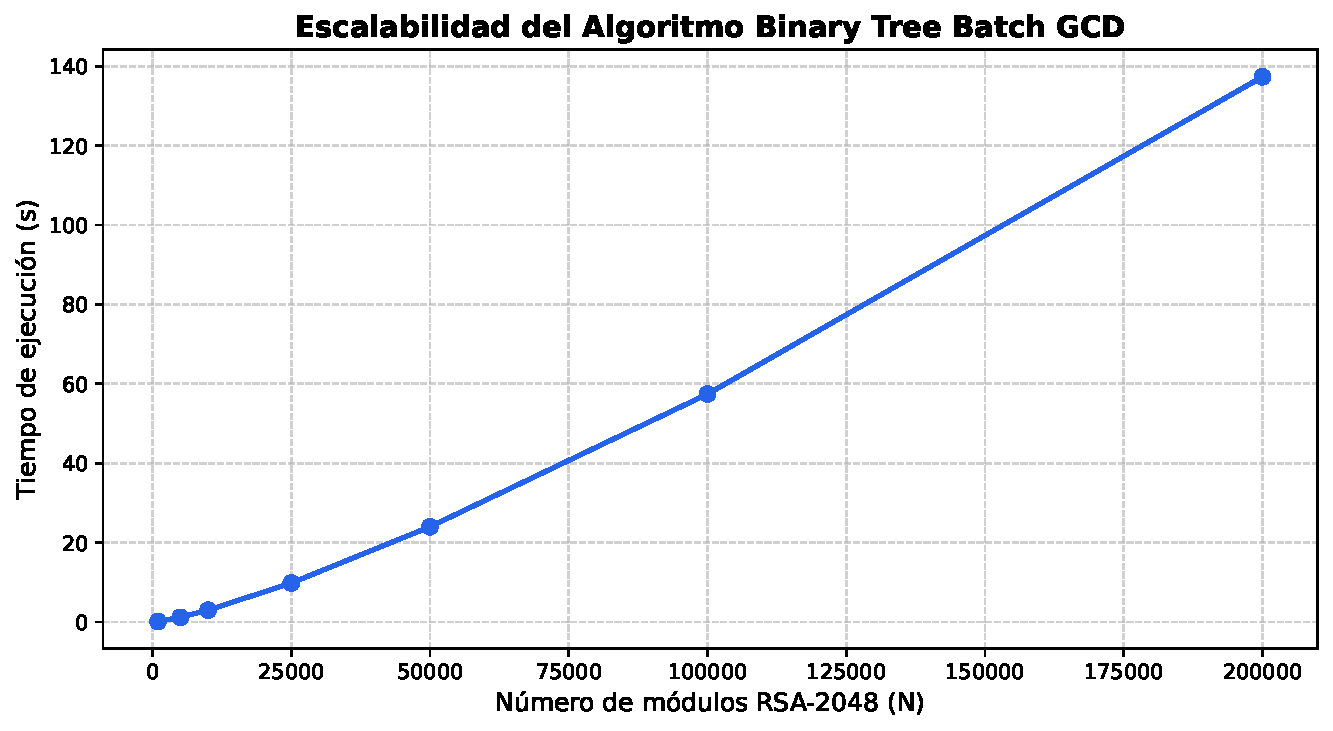
\includegraphics[width=0.78\textwidth]{escalabilidad_batch_gcd.pdf}
    \caption{Tiempo de ejecución del algoritmo sobre conjuntos de claves sintéticas de tamaño creciente.}
    \label{fig:synthetic_scalability}
\end{figure}

A partir de esta gráfica puede observarse que el tiempo de ejecución aumenta de forma progresiva conforme crece el tamaño del conjunto de módulos analizados. Este resultado era esperable, ya que la construcción del árbol de productos y la fase final de enumeración dependen directamente del número de entradas procesadas. No obstante, lo relevante en este punto no es solo que el tiempo aumente, sino que lo haga de una forma suficientemente controlada como para considerar viable el uso del algoritmo sobre conjuntos mayores.
\\
\\
En este sentido, los resultados obtenidos en esta primera fase pueden considerarse positivos. Por un lado, la implementación detectó correctamente los casos en los que se habían introducido factores compartidos de forma artificial. Por otro, la evolución temporal observada en la gráfica sugiere que el algoritmo mantiene un comportamiento razonable al escalar el tamaño de entrada, al menos dentro del rango de valores analizado en esta fase experimental.
\\
\\
Conviene señalar, no obstante, que estas pruebas sintéticas tienen un alcance limitado. Al tratarse de datos generados de manera controlada, no reproducen toda la complejidad que puede aparecer en conjuntos reales de claves públicas. En particular, no recogen la diversidad estructural de los certificados presentes en \textit{CT logs}, ni la posible aparición de casos más irregulares o menos frecuentes de factores compartidos.
\\
\\
Aun así, esta primera fase cumple una función metodológica importante dentro del trabajo. Nos permite verificar que la implementación es correcta, disponer de una primera medida de su comportamiento temporal y justificar el paso a una segunda etapa de análisis sobre datos reales. En otras palabras, los experimentos sintéticos actúan como una validación inicial necesaria antes de aplicar el algoritmo a módulos RSA extraídos de \textit{Certificate Transparency logs}.

\section{Resultados preliminares sobre datos reales}

Una vez validado el comportamiento de la implementación sobre datos sintéticos, la siguiente fase del trabajo consistió en aplicar el algoritmo sobre una muestra de datos reales obtenida a partir de \textit{Certificate Transparency logs}. El objetivo de esta etapa no ha sido todavía realizar una auditoría completa sobre todos los \textit{CT logs}, sino comprobar que el procedimiento desarrollado puede ejecutarse correctamente también en un entorno real y observar su comportamiento inicial fuera del escenario controlado de los experimentos sintéticos.
\\
\\
Para ello, en el notebook se implementó un pequeño \textit{pipeline} de extracción de certificados X.509 desde la API pública de Certificate Transparency. En esta fase se utilizó el log público \textit{Argon 2025h2} de Google y se descargó una muestra de 20.000 entradas. A partir de esas entradas se decodificaron los certificados contenidos en formato DER, se filtraron únicamente aquellas claves públicas RSA de exactamente 2048 bits y, finalmente, se extrajeron sus módulos en formato hexadecimal. Tras eliminar duplicados, el conjunto resultante quedó formado por 20.000 módulos RSA-2048 únicos, almacenados en el archivo \texttt{real\_moduli.txt}.
\\
\\
La propia salida del notebook confirma que, durante esta fase de extracción, se procesaron correctamente las 20.000 entradas previstas, que no se produjeron errores al decodificar certificados y que el archivo final contenía exactamente 20.000 módulos válidos. Este resultado es importante porque garantiza que la prueba posterior del algoritmo se realizó sobre una muestra limpia y homogénea de claves RSA reales.
\\
\\
Una vez generado el archivo de entrada, se ejecutó el binario \texttt{batch\_gcd\_real} desarrollado en C++ con la misma lógica de las tres fases ya descritas: construcción del árbol de productos con \textit{gcd} en línea, agregación en la variable \(B\) y enumeración final sobre el conjunto original. La ejecución se realizó empleando 10 hilos de OpenMP, tal como aparece en la salida del experimento registrada en el notebook.
\\
\\
Los resultados obtenidos en esta primera prueba real fueron los siguientes. En la fase de carga se leyeron correctamente los 20.000 módulos del archivo, verificándose además que tanto el primer como el último módulo tenían 2048 bits. El tiempo dedicado a esta fase fue de 47,91 ms.
\\
\\
Durante la Fase 1, correspondiente a la construcción del árbol de productos y al cálculo de \textit{gcd} en línea, el algoritmo construyó 15 niveles del árbol y no encontró ningún \textit{gcd} no trivial. El tiempo empleado en esta fase fue de 7058,81 ms.
\\
\\
En la Fase 2, dedicada a la agregación de divisores comunes en la variable \(B\), el resultado fue un entero de longitud 1 bit, es decir, \(B = 1\). Esto indica que la fase anterior no había encontrado ningún divisor común no trivial dentro del conjunto analizado. El tiempo consumido en esta etapa fue prácticamente nulo.
\\
\\
Por último, en la Fase 3 de enumeración final, el algoritmo no detectó ninguna clave vulnerable, obteniéndose un total de 0 claves con factores compartidos. El tiempo invertido en esta fase fue de 0,88 ms. En conjunto, el tiempo total de ejecución del algoritmo sobre esta muestra real fue de 7059,70 ms, es decir, aproximadamente 7,06 segundos.
\\
\\
Desde el punto de vista de la interpretación de resultados, este experimento ofrece varias conclusiones relevantes. En primer lugar, confirma que la implementación desarrollada puede aplicarse sin problemas a una muestra real de claves RSA obtenidas de \textit{CT logs}, manteniendo la misma estructura algorítmica utilizada en los experimentos sintéticos. En segundo lugar, el hecho de no haber encontrado claves vulnerables en esta muestra concreta no debe interpretarse como una contradicción respecto a los trabajos previos, sino como un resultado compatible con el tamaño reducido del subconjunto analizado.
\\
\\
Además, conviene tener presente que esta prueba se ha realizado sobre una muestra todavía muy pequeña en comparación con la escala del problema completo. Tal y como se vio en el capítulo anterior, tanto la tesis de Våge como otros trabajos previos trabajaron con decenas o cientos de millones de claves para detectar casos poco frecuentes de factores compartidos. Por ello, el hecho de que en esta muestra de 20.000 módulos no hayan aparecido vulnerabilidades no resulta sorprendente y no invalida en absoluto el interés del enfoque.
\\
\\
Lo importante en esta fase no era tanto obtener ya un hallazgo positivo, sino comprobar que el procedimiento completo de extracción, filtrado y análisis funciona correctamente sobre datos reales. En este sentido, el experimento puede considerarse satisfactorio: la muestra se generó correctamente, la implementación procesó sin errores los 20.000 módulos y el comportamiento temporal observado fue razonable para este tamaño de entrada.
\\
\\
Por tanto, esta primera prueba sobre datos reales debe entenderse como una validación inicial del método en un entorno práctico. Aunque todavía no representa el análisis masivo de los \textit{CT logs} que constituye el objetivo más ambicioso del trabajo, sí establece una base experimental útil sobre la que podrán plantearse futuras ampliaciones a conjuntos de tamaño mucho mayor.